\documentclass[11pt]{article}

\usepackage{fullpage}
\usepackage{rotating}   
\usepackage{amsmath}
\usepackage{amssymb}
\usepackage{amsthm}
\usepackage{fancyhdr}
\usepackage{algorithm}
\usepackage{algorithmic}
\usepackage{bm}
\usepackage{listings}
\usepackage{graphicx}
\usepackage{caption2}
\usepackage{subfigure}
\usepackage{float}
\usepackage{extpfeil}
\usepackage{color}
\usepackage[usenames,dvipsnames]{xcolor}


\newtheorem{theorem}{Theorem}[section]
\newtheorem{lemma}[theorem]{Lemma}
\newtheorem{corollary}[theorem]{Corollary}
\newtheorem{proposition}[theorem]{Proposition}
\newtheorem{definition}[theorem]{Definition}
\newtheorem{conjecture}[theorem]{Conjecture}
\newtheorem{remark}[subsection]{Remark}

%%
\newcommand\numberthis{\addtocounter{equation}{1}\tag{\theequation}}

%% define new symbols
\def\bx{\bm{x}}
\def\bb{\bm{b}}
\def\ba{\bm{a}}
\def\bc{\bm{c}}
\def\bf{\bm{f}}
\def\by{\bm{y}}
\def\bu{\bm{u}}
\def\bv{\bm{v}}
\def\BW{\bm{W}}
\def\BA{\bm{A}}
\def\bz{\bm{z}}
\def\BZ{\bm{Z}}
\def\BH{\bm{H}}
\def\BL{\bm{L}}
\def\BU{\bm{U}}
\def\BV{\bm{V}}
\def\BB{\bm{B}}
\def\BC{\bm{C}}
\def\BD{\bm{D}}
\def\BE{\bm{E}}
\def\BW{\bm{W}}
\def\BQ{\bm{Q}}
\def\BG{\bm{G}}
\def\BA{\bm{A}}
\def\BX{\bm{X}}
\def\BY{\bm{Y}}
\def\BQ{\bm{Q}}
\def\BI{\bm{I}}
\def\BR{\bm{R}}

%% define new brackets
\def\la{\left\langle}
\def\ra{\right\rangle}
\def\ln{\left\|}
\def\rn{\right\|}
\def\lb{\left(}
\def\rb{\right)}
\def\lsb{\left[}
\def\rsb{\right]}
\def\lcb{\left\{}
\def\rcb{\right\}}

%%
\DeclareMathOperator*{\argmin}{arg\,min}
\DeclareMathOperator*{\argmax}{arg\,max}

%%
\title{Homework VIII}
\author{Name: Shao Yanjun, Number: 19307110036}


\begin{document}
\maketitle

%------------------------------------
\begin{abstract}
This is Daniel's homework of  "Numerical Algorithms with Case Studies II".
\end{abstract}
%-------------------------------------
%=====================
\section{Problems}
\paragraph{Q1}
Use the short recurrence formula for Chebyshev polynomial $2x\tilde{\omega_n}(x)=\tilde{\omega_{n+1}}+\tilde{\omega_{n-1}}$, we can calculate the eigenvalues of the following matrix to get $n$ Chebyshev points.
\begin{align}
	\lambda_k
	\begin{pmatrix}
		\tilde{\omega_0}(\lambda_k)\\
		\tilde{\omega_1}(\lambda_k)\\
		\tilde{\omega_2}(\lambda_k)\\
		\vdots\\
		\tilde{\omega_{n-2}}(\lambda_k)\\
		\tilde{\omega_{n-1}}(\lambda_k)
	\end{pmatrix}
=
	\begin{pmatrix}
		0 & 1 & 0 & \cdots &0 &0 &0\\
		1 & 0 & 1 & \cdots &0 &0 &0\\
		0 & 1 & 0 & \cdots &0 &0 &0\\
		\vdots & \vdots &\vdots &\ddots &\vdots & \vdots &\vdots\\
		0 &0 &0 &\cdots & 1 & 0 & 1\\
		0 &0 &0 &\cdots & 0 & 1 & 0&
	\end{pmatrix}
	\begin{pmatrix}
		\tilde{\omega_0}(\lambda_k)\\
		\tilde{\omega_1}(\lambda_k)\\
		\tilde{\omega_2}(\lambda_k)\\
		\vdots\\
		\tilde{\omega_{n-2}}(\lambda_k)\\
		\tilde{\omega_{n-1}}(\lambda_k)
	\end{pmatrix}
\end{align}
Use lemma for symmetric tridiagonal matrices, or rather the known Chebyshev points, we can calculate nodes that $\lambda_i=cos(\dfrac{(2i-1)\pi}{2n})$.\\
Next, we will calculate the coefficients $A_i$ for the approximation  $\int_{-1}^{1}\dfrac{1}{\sqrt{1-x^2}}f(x)\mathrm{d}x\approx\sum_{i=1}^{n}A_if(cos(\dfrac{(2i-1)\pi}{2n}))$.
Construct a Langrangian basis polynomial, $p_i(x)=\prod_{j\ne i}^{n}(x-\lambda_i)$. \\We must have $\int_{-1}^{1}\dfrac{1}{\sqrt{1-x^2}}\tilde{\omega_{n-1}}(x)p_i(x)\mathrm{d}x=A_i\tilde{\omega_{n-1}}(\lambda_i)p_i(\lambda_i)=\int_{-1}^{1}\dfrac{1}{\sqrt{1-x^2}}\tilde{\omega^2_{n-1}}(x)\mathrm{d}x$, because $\mathbf{deg}p(x)=2n-2$ is in the exactness bound, and $\langle\tilde{\omega_{n-1}}(x),p_i(x)\rangle_{\rho(x)}=\langle\tilde{\omega_{n-1}}(x),\tilde{\omega_{n-1}}(x)\rangle_{\rho(x)}.$
Therefore,
\begin{align}
	A_i&=\frac{\langle\tilde{\omega_{n-1}}(x),\tilde{\omega_{n-1}}(x)\rangle_{\rho(x)}}{\tilde{\omega_{n-1}}(\lambda_k)\cdot\tilde{\omega'_{n}}(\lambda_k)}\\
	&=\frac{\frac{\pi}{2}}{cos((n-1)arccos(cos(\frac{(2i-1)\pi}{2n})))(-\frac{n}{sin(\frac{(2i-1)\pi}{2n})}sin(narccos(cos(\frac{(2i-1)\pi}{2n}))))}\\
	&=\frac{\pi}{n}
\end{align}
So, the quadrature rule reads $\int_{-1}^{1}\dfrac{1}{\sqrt{1-x^2}}f(x)\mathrm{d}x\approx\sum_{i=1}^{n}\dfrac{\pi}{n}f(cos(\dfrac{(2i-1)\pi}{2n}))$
\paragraph{Q2}
\paragraph{Q3}
The integral area is symmetric on $x,y$,
\begin{figure}[H]
	\centering
	\subfigure[integral area]{
		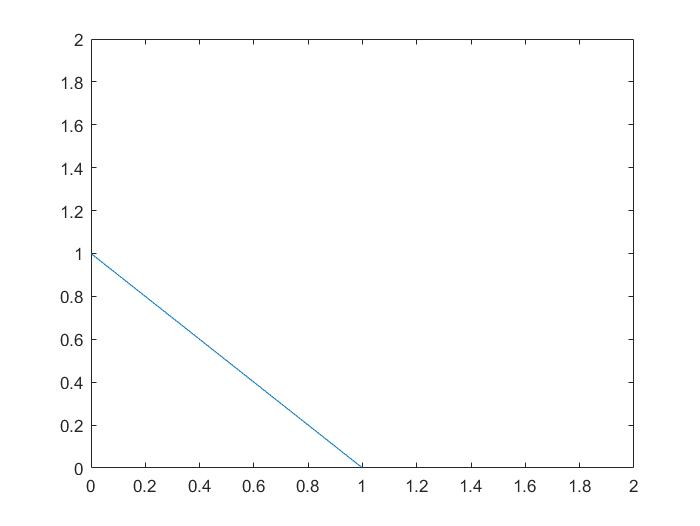
\includegraphics[width=0.6\linewidth]{area.jpg}
	}
\end{figure}
Evaluate $\int_{0}^{1}\int_{0}^{1-y}f(x,y)\mathrm{d}x\mathrm{d}y$,
\begin{align*}
	&\int_{0}^{1}\int_{0}^{1-y}\mathrm{d}x\mathrm{d}y=\int_{0}^{1}1-y\mathrm{d}y=\frac{1}{2}=\frac{1}{6}(f(\frac{1}{2},0)+f(0,\frac{1}{2})+f(\frac{1}{2},\frac{1}{2}))=\frac{1}{6}(f(\frac{2}{3},\frac{1}{6})+f(\frac{1}{6},\frac{2}{3})+f(\frac{1}{6},\frac{1}{6}))\\
	&\int_{0}^{1}\int_{0}^{1-y}x\mathrm{d}x\mathrm{d}y=\int_{0}^{1}\int_{0}^{1-y}y\mathrm{d}x\mathrm{d}y=\frac{1}{6}=\frac{1}{6}(f(\frac{1}{2},0)+f(0,\frac{1}{2})+f(\frac{1}{2},\frac{1}{2}))=\frac{1}{6}(f(\frac{2}{3},\frac{1}{6})+f(\frac{1}{6},\frac{2}{3})+f(\frac{1}{6},\frac{1}{6}))\\
	&\int_{0}^{1}\int_{0}^{1-y}x^2\mathrm{d}x\mathrm{d}y=\int_{0}^{1}\int_{0}^{1-y}y^2\mathrm{d}x\mathrm{d}y=\frac{1}{12}=\frac{1}{6}(f(\frac{1}{2},0)+f(0,\frac{1}{2})+f(\frac{1}{2},\frac{1}{2}))=\frac{1}{6}(f(\frac{2}{3},\frac{1}{6})+f(\frac{1}{6},\frac{2}{3})+f(\frac{1}{6},\frac{1}{6}))\\
	&\int_{0}^{1}\int_{0}^{1-y}xy\mathrm{d}x\mathrm{d}y=\frac{1}{24}=\frac{1}{6}(f(\frac{1}{2},0)+f(0,\frac{1}{2})+f(\frac{1}{2},\frac{1}{2}))=\frac{1}{6}(f(\frac{2}{3},\frac{1}{6})+f(\frac{1}{6},\frac{2}{3})+f(\frac{1}{6},\frac{1}{6}))\\
	&\int_{0}^{1}\int_{0}^{1-y}x^3\mathrm{d}x\mathrm{d}y=\int_{0}^{1}\int_{0}^{1-y}y^3\mathrm{d}x\mathrm{d}y=\frac{1}{20}\ne \frac{1}{6}(f(\frac{1}{2},0)+f(0,\frac{1}{2})+f(\frac{1}{2},\frac{1}{2}))\ne \frac{1}{6}(f(\frac{2}{3},\frac{1}{6})+f(\frac{1}{6},\frac{2}{3})+f(\frac{1}{6},\frac{1}{6}))\\
	&\int_{0}^{1}\int_{0}^{1-y}x^2y\mathrm{d}x\mathrm{d}y=\int_{0}^{1}\int_{0}^{1-y}xy^2\mathrm{d}x\mathrm{d}y=\frac{1}{60}\ne \frac{1}{6}(f(\frac{1}{2},0)+f(0,\frac{1}{2})+f(\frac{1}{2},\frac{1}{2}))\ne\frac{1}{6}(f(\frac{2}{3},\frac{1}{6})+f(\frac{1}{6},\frac{2}{3})+f(\frac{1}{6},\frac{1}{6}))
\end{align*}
Therefore, the maximum exactness is quadratic.
\paragraph{Q4}
The integral area should be partitioned as follows recursively,
\begin{figure}[H]
	\centering
	\subfigure[integral area]{
		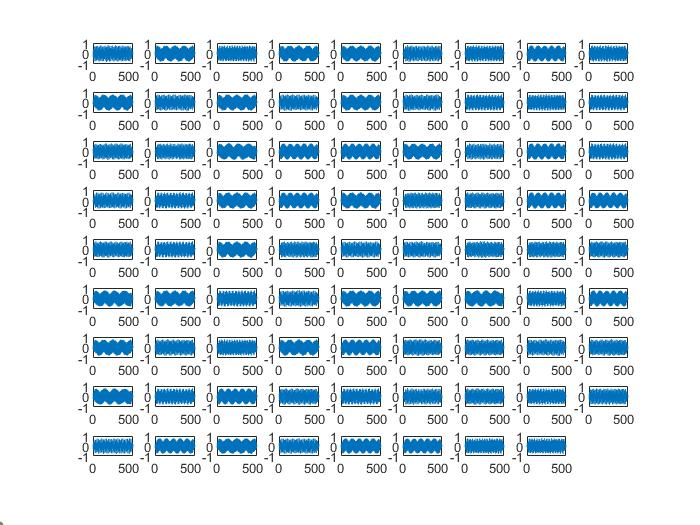
\includegraphics[width=0.6\linewidth]{division.jpg}
	}
\end{figure}
Where the colored triangles will use reversed formula, while uncolored triangles will directly apply the $2^{nd}$ formula given in Q3.
\begin{figure}[H]
	\centering
	\subfigure[Result]{
		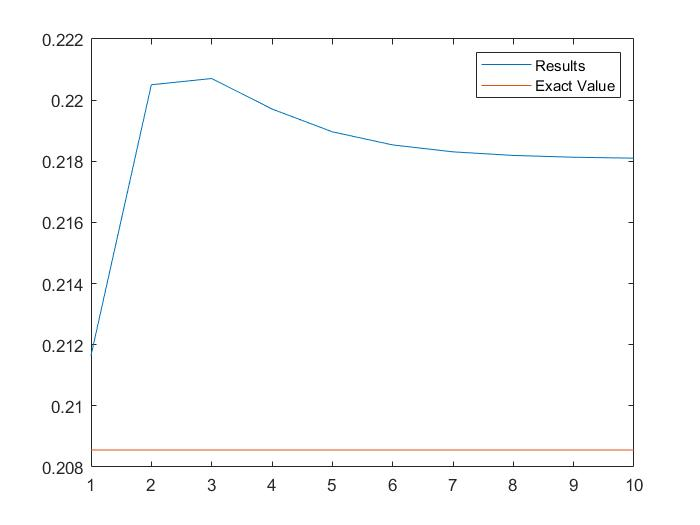
\includegraphics[width=0.6\linewidth]{Result.jpg}
	}
\end{figure}
Curiously, the result doesn't seem to converge to the exact value $\dfrac{1}{2}(cos(1) + e - sin(1)) - 1$.
\paragraph{Q5}
It seems we can do a substitution on variables that $u=x^2,v=y^2$, so that the integration becomes $\int\int_{x^2+y^2\le1}e^xsin(y)\mathrm{d}x\mathrm{d}y=\int_{0}^{1}\int_{0}^{1-v}e^{\sqrt{u}}sin(\sqrt{v})\dfrac{1}{4\sqrt{uv}}\mathrm{d}x\mathrm{d}y$. Use the same code now, and the result is $0.47125$.
\begin{figure}[H]
	\centering
	\subfigure[Result]{
		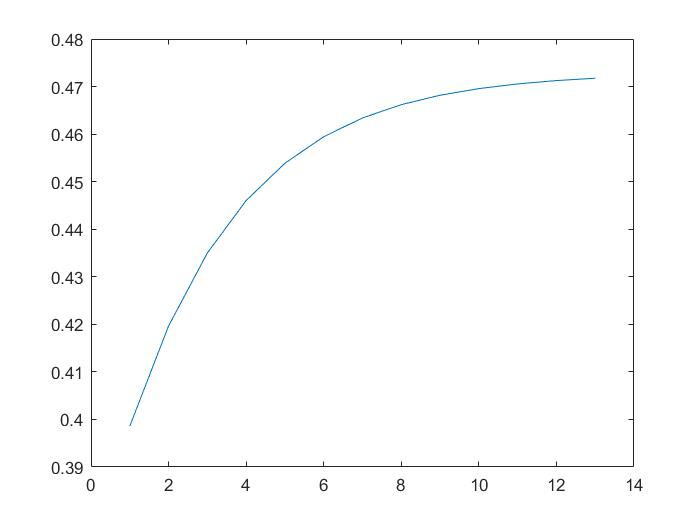
\includegraphics[width=0.6\linewidth]{Result5.jpg}
	}
\end{figure}
%-------------------------------------
%=====================
\end{document}
